
% ----------------------------------------------------------------------------------------------------
\section{Introduction}

\begin{figure}[t]
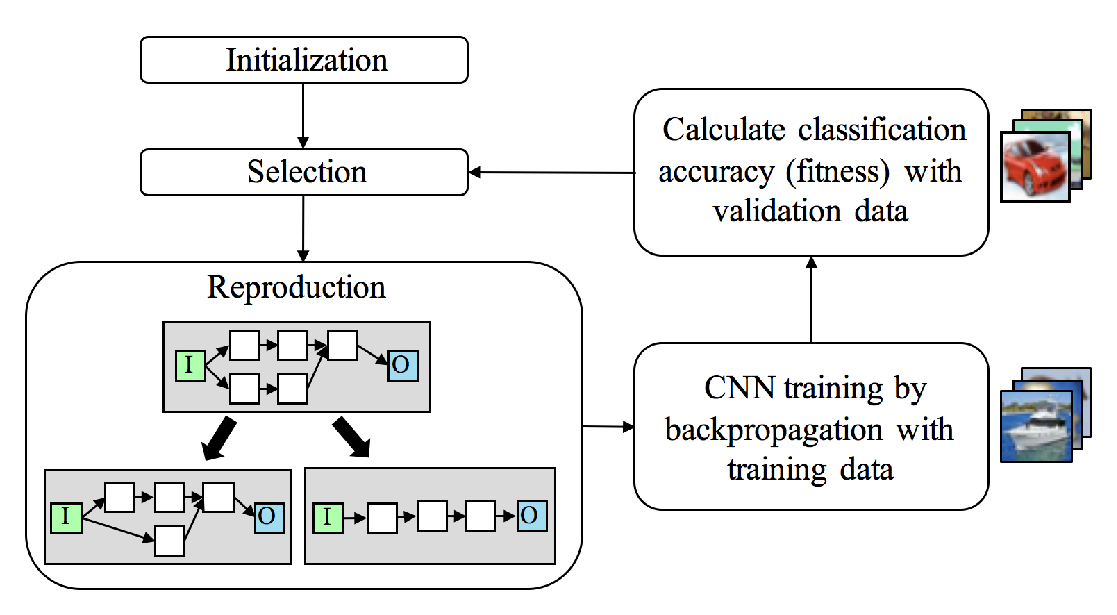
\includegraphics[scale=0.45]{images/overview.eps}
\caption{Overview of our method. Our method searches a CNN architecture using genetic programming. That CNN architecture is then trained on a learning task, and returns an accuracy. The network search is performed to maximize the accuracy by the evolutionary algorithm.}
\label{overview}
\end{figure}

Deep learning, which uses deep neural networks as a model, has shown a good performance on many challenging artificial intelligence and machine learning tasks such as image recognition \cite{lecun_gradient-based_1998,krizhevsky_imagenet_2012}, speech recognition \cite{hinton_deep_2012}, and reinforcement learning tasks \cite{mnih_playing_2013,mnih_human-level_2015}.
In particular, convolutional neural networks (CNNs) \cite{lecun_gradient-based_1998} have seen huge success in image recognition tasks in the last few years and is applied to various computer vision application, e.g. GAN \cite{goodfellow_generative_2014}, colorization \cite{zhang_colorful_2016}, image to text anotation \cite{vinyals_show_2015}.
A commonly used CNN architecture mainly consists of several convolutions, pooling, and fully connected layers.
Several recent studies focus on developing the novel CNN architecture that achieves higher classification accuracy, e. g., GoogleNet \cite{szegedy_going_2015}, ResNet \cite{he_deep_2016}, and DensNet \cite{huang_densely_2016}.
Despite their success, designing CNN architectures is still a difficult task since there exist many design parameters such as the depth of a network, the type and parameters of each layer, and the connectivity of the layers.
The state-of-the-art CNN architectures have become deep and complex, which suggests that a significant number of design parameters should be tuned to realize the best performance for a specific dataset.
Therefore, the trial and error or expert knowledge are required when the users construct the suitable architecture for their target dataset.
Because of this situation, the automatic design methods for the CNN architectures is highly beneficial.

The neural network architecture design can be viewed as the model selection problem in the machine learning. The straight-forward approach is to deal with the architecture design as the hyperparameter optimization problem, optimizing the hyperparameters such as the number of layers and neurons using black-box optimization techniques \todo{\cite{}.}

Evolutionary computation has been traditionally applied to design the neural network architectures \todo{ref. X. Yao's review, Kitano, etc...}.
There are two types of encoding schemes for the network representation: direct and indirect coding.
The direct coding represents the number and connectivity of neurons directly as the genotype, whereas the indirect coding represents a generation rule of the network architectures.
While almost traditional approaches optimize the number and connectivity of low-level neurons, the modern neural network architectures for deep learning have many units and various types of units, e.g., convolution, pooling, and normalization.
Optimizing those many parameters in reasonable computational time may be difficult.
Therefore, the use of the highly-functional modules as a minimum unit is promising.

In this paper, we attempt to design CNN architectures based on a genetic programming.
We use the Cartesian genetic programming (CGP) \cite{miller_cartesian_2000,harding_evolution_2008} encoding scheme, one of the direct encoding, to represent the CNN structure and connectivity.
The advantage of this representation is its flexibility; it can represent variable-length network structure and the skip connections.
Moreover, we adopt the relatively highly-functional modules such as convolutional blocks and tensor concatenation as the node functions in CGP to reduce the search space.
To evaluate the architecture represented by the CGP, we train the network using training dataset in an ordinary way. Then the performance for another validation dataset is assigned as the evaluation of the architecture. Based on this fitness evaluation, an evolutionary algorithm optimizes the CNN architectures.
 To check the performance of the proposed approach, we conducted the experiment constructing the CNN architecture for the image classification task with the CIFAR-10 dataset \cite{krizhevsky_learning_2009}. The experimental result shows that the proposed approach can automatically find the competitive CNN architecture compared with state-of-the-art models.

\shin{It would be nice if we can describe the research question clearly.}

The rest of this paper is organized as follows. The next section presents related work on the neural network architecture design. In Section 3, we describe our genetic programming approach to design the CNN architectures. We test the performance of the proposed approach through the experiment. Finally, in Section 5, we describe our conclusion and future work.


\begin{figure*}[t]
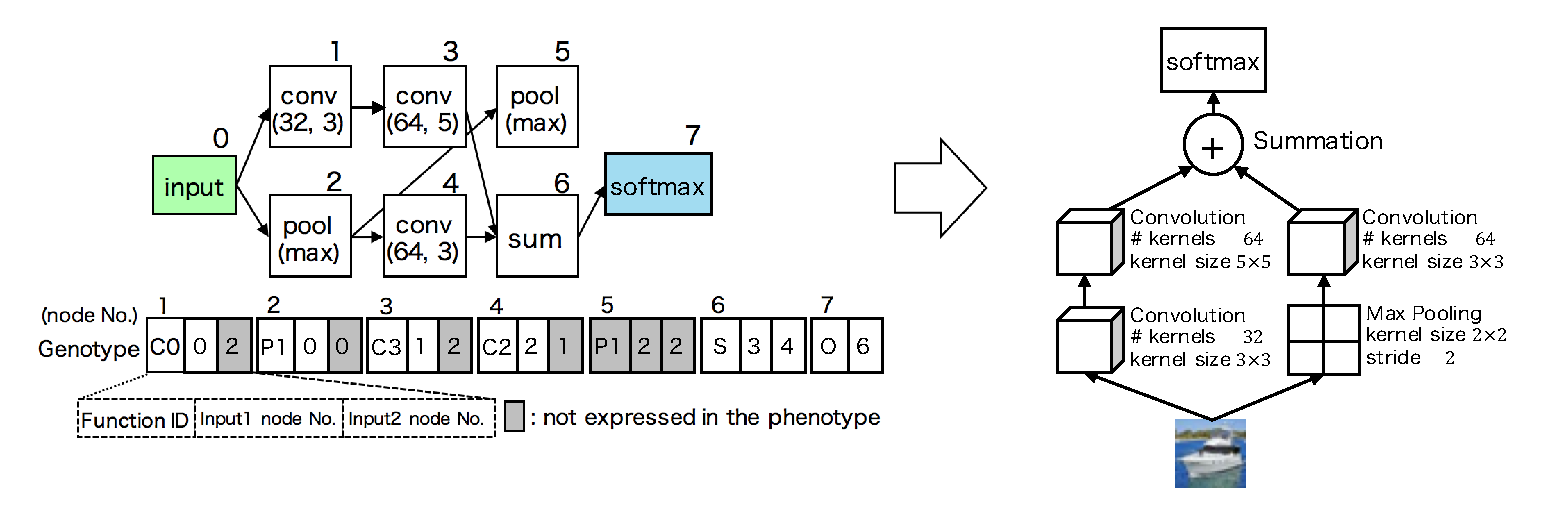
\includegraphics[scale=0.65]{images/genotype.eps}
\caption{Example of a genotype and a phenotype. The genotype (Left) defines a CNN architecture (Right).}
\label{genotype}
\end{figure*}
% ----------------------------------------------------------------------------------------------------
\section{Related Work}
%Automating neural network design and hyperparameter optimization are important topic in machine learning.
This section briefly reviews the related work on the automatic neural network architecture design: hyperparameter optimization, evolutionary neural networks, and reinforcement learning approach.

\subsection{Hyperparameter Optimization}
We can consider the neural network architecture design as the model selection or hyperparameter optimization problem from machine learning perspective. There are many hyperparameter tuning methods for the machine learning algorithm such as grid search, gradient search \cite{bengio_gradient-based_2000}, random search \cite{bergstra_random_2012}, and Bayesian optimization based methods \cite{hutter_sequential_2011,snoek_practical_2012}. Naturally, evolutionary algorithms have also been applied to the hyperparameter optimization problems \todo{\cite{} \cite{CMA etc...}.} In the machine learning community, Bayesian optimization is often used and have shown good performance in several datasets. Bayesian optimization is a global optimization method of black-box and noisy objective functions, which maintains a surrogate model learned by using previously evaluated solutions. A Gaussian process is usually adopted as the surrogate model \cite{snoek_practical_2012}, which can easily handle the uncertainty and noise of the objective function.
Bergstra et al. \cite{bergstra_algorithms_2011} have proposed the Tree-structured Parzen estimator (TPE) and shown better results than manual search and random search \cite{bergstra_random_2012}.
They have also proposed a meta-modeling approach \cite{bergstra_making_2013} based on the TPE for supporting automatic hyperparameter optimization. 
Snoek et al. \cite{snoek_scalable_2015} used a deep neural network instead of the Gaussian process to reduce the computational cost for the surrogate model building and succeeded to improve the scalability.

The hyperparameter optimization approach often tunes the predefined hyperparameters such as the number of layers and neurons, and the type of activation functions. While this method has seen success, it is hard to design more flexible architectures from scratch.

\subsection{Evolutionary Neural Networks}
Evolutionary algorithms have been used to optimize the neural network architectures so far \cite{schaffer_combinations_1992,stanley_evolving_2002}. The traditional approaches are not suitable for the model deep neural network architecture design since they usually optimize the number and connectivity of low-level neurons.

Recently, Fernando et al. \cite{fernando_convolution_2016} have proposed the differentiable pattern-producing networks (DPPNs) to optimize weights of a denoising autoencoder. The DPPN is a differentiable version of the compositional pattern-producing networks (CPPNs) \cite{stanley_compositional_2007}. This method focuses on the effectiveness of the indirect coding for weight optimization. That is, the general structure of network should be predefined.

Verbancsics et al. \cite{verbancsics_generative_2013,verbancsics_image_2015} have designed the artificial neural networks and CNN architectures with the hypercube-based neuroevolution of augmenting topologies (HyperNEAT) \cite{stanley_hypercube-based_2009}.
However, to the best of our knowledge, these networks designed with HyperNEAT have failed to match the performance of state-of-the-art methods \shin{I do not know the contents of Verbancsics's papers}.
Also, these methods deal with the architectures defined by human experts. Thus it is hard to design neural network architectures from scratch.

\subsection{Reinforcement Learning Approach}
The interesting approaches, automatic designing the deep neural network architecture using reinforcement learning, have been attempted recently \cite{zoph_neural_2016,baker_designing_2016}.
These studies showed that a reinforcement learning based method could construct the competitive CNN architectures for image classification tasks.
In \cite{zoph_neural_2016}, a recurrent neural network (RNN) is used to generate the neural network architectures, and the RNN is trained with reinforcement learning to maximize the expected accuracy on a learning task.
This method uses distributed training and asynchronous parameter updates with $800$ GPUs to accelerate the reinforcement learning process.
Baker et al. \cite{baker_designing_2016} have proposed a meta-modeling approach based on reinforcement learning to produce the CNN architectures.
A Q-learning agent explores and exploits a space of model architectures with an $\epsilon -$greedy strategy and experience replay.

These approaches adopt the indirect coding scheme for the network representation, which optimizes generative rules for the network architectures such as the RNN.
Unlike these approaches, our approach uses the direct coding based on Cartesian genetic programming to design the CNN architectures.
Besides, we introduce the relatively highly-functional modules such as convolutional blocks and tensor concatenations to find better CNN architectures efficiently.


% ----------------------------------------------------------------------------------------------------
\section{CNN Architecture Design Using Cartesian Genetic Programming}
Our method directly encodes the CNN architectures based on CGP and uses the highly-functional modules as the node functions.
The CNN architecture defined by the CGP is trained using training dataset, followed by the validation accuracy is assigned as the fitness of the architecture. Then the architecture is optimized to maximize the validation accuracy by the evolutionary algorithm.
Figure \ref{overview} illustrates the overview of our method.

In this section, we describe the network representation and the evolutionary algorithm used in the proposed method in detailed.

\subsection{Representation of CNN Architectures}
We use the CGP encoding scheme, representing the program as the form of directed acyclic graphs with a two-dimensional grid defined on computational nodes, for the CNN architecture representation. Let assume the grid has $N_r$ rows by $N_c$ column, then the number of intermediate nodes is $N_r \times N_c$, and the numbers of inputs and outputs depend on the task. The genotype consists of the integers with fixed length, and each gene has the information of the type and connections of the node. The $r$th column's nodes should be connected from the $r-l$ to $r-1$th column's nodes, where $l$ is called levels-back parameter. Figure \ref{genotype} shows an example of the genotype, the corresponding network and CNN architecture in the case of two rows by three columns. While the genotype in CGP is a fixed length representation, the number of nodes in the phenotypic network varies since not all the nodes are not connected to the output node. The node No. 5 in the left of Figure \ref{genotype} is inactive nodes.

Referring the modern CNN architectures, we select the highly-functional modules as the node function.
The frequently-used processings in the CNN are convolution and pooling; convolution processing uses a local connectivity and spatially shares the learnable weights, and pooling is nonlinear down-sampling.
We prepare the six types of node functions called ConvBlock, ResBlock, max-pooling, average-pooling, tensor concatenation, and tensor summation.

The ConvBlock consists of a standard convolution processing followed by batch normalization \cite{ioffe_batch_2015} and rectified linear units (ReLU) \cite{nair_rectified_2010}. In the ConvBlock, we pad the outside of the input feature map with zero values before the convolution operation so as to keep the size of the output. 
As a result, the $M \times N \times C$ input feature map is transformed into the $M \times N \times C'$ output, where $M$, $N$, $C$, and $C'$ are the numbers of rows, columns, input channels, and output channels of a convolution layer, respectively.

The ResBlock is composed of a convolution processing, batch normalization, ReLU, and element-wise addition.
A ResBlock architecture is shown in Figure \ref{resblock}.
The ResBlock performs identity mapping by shortcut connections described in \cite{he_deep_2016}.
The input size is preserved in the same way as ConvBlock after convolution.
Output feature maps of the ResBlock are calculated by ReLU and element-wise addition of input feature maps and output feature maps of the stacked layers as seen in Figure \ref{resblock}.
In the ResBlock, the $M\times N\times C$ input feature map is transformed into the $M\times N\times C'$ output.

The max- and average-pooling use the maximum and average values as the values of the down-sampled images, respectively.
In the pooling operation, the $M \times N \times C$ input feature map is transformed into the $M' \times N' \times C$ output, where $M' = M/2$ and $N' = N/2$.

The tensor concatenation concatenates two feature maps in the depth dimensions.
If the input feature maps to be concatenated have the different number of rows or column, we down-sample the larger feature map by max-pooling so as to become the same sizes of inputs.
In the concatenation operation, the size of the output feature map is $\min (M_1, M_2) \times \min (N_1, N_2) \times C_1 + C_2$, where the sizes of the inputs are $M_1 \times N_1 \times C_1$ and $M_2 \times N_2 \times C_2$.

The tensor summation performs element-wise addition of two feature maps, channel by channel. 
In the same way as concatenation, if the input feature maps to be added have the different number of rows or columns, we down-sample the larger feature map by max-pooling.
Besides, if the inputs have the different number of channels, we pad the smaller feature map with zeros for increasing channels.
In the summation operation, the size of the output feature map is $\min (M_1, M_2) \times \min (N_1, N_2) \times \max (C_1, C_2)$, where the sizes of the inputs are $M_1 \times N_1 \times C_1$ and $M_2 \times N_2 \times C_2$.

Adding these summation and concatenation operations allows our method to represent shortcut connections or branching layers such as used in GoogleNet \cite{szegedy_going_2015} and Residual Net \cite{he_deep_2016}.
The output node represents softmax function with the number of classes.
The node functions used in the experiments are displayed in Table \ref{layer_param}.


\begin{table}[tb]
  \caption{Parameter details for each layer}
  \label{layer_param}
  \begin{tabular}{l|l|l} \hline
    Node type & Parameters & Values or description \\ \hline
    ConvBlock & Receptive field size & $\in \{3\times 3, 5\times 5\}$ \\ 
                        & \# kernels & $\in \{32, 64, 128\}$ \\ 
                       & Stride & $1$ \\ 
                       & \# inputs & $1$ \\ \hline
    ResBlock & Receptive field size & $\in \{3\times 3, 5\times 5\}$ \\ 
                        & \# kernels & $\in \{32, 64, 128\}$ \\ 
                       & Stride & $1$ \\ 
                       & \# inputs & $1$ \\ \hline
      Pooling     & Receptive field size & $2\times 2$ \\ 
                       & Stride & $2$ \\ 
                       & \# inputs & $1$ \\ \hline
     Summation & \# inputs & $2$ \\ 
                         &                & Element-wise addition. \\ \hline
 Concatenation & \# inputs & $2$ \\ 
                      &  & Concatenate in the \\
                       &  & depth dimension.\\  \hline
  \end{tabular}
\end{table}


\subsection{Evolutionary Algorithm}
We use a point mutation as the genetic operator as same as the standard CGP. The type and connections of each node randomly change to valid values according to a mutation rate. 
The standard CGP mutation has a possibility only to affect the inactive node. In that case, the phenotype (representing CNN architecture) does not change by the mutation and does not need fitness evaluation again.

The fitness evaluation of the CNN architectures is so expensive since it requires the training of CNN.
To efficiently use the computational resource, we want to evaluate some candidate solutions in parallel at each generation.
Therefore, we apply the mutation operator until at least one active node changes to reproduce the candidate solution. We call this mutation as forced mutation.
Moreover, to keep a neutral drift, which is effective for CGP evolution \todo{\cite{}}, we modify a parent by the neutral mutation if the fitnesses of the offsprings do not improve.
Here, the neutral mutation only changes the genes of inactive nodes without modification of the phenotype.

We use the modified $(1+\lambda)$ evolutionary strategy (with $\lambda = 2$ in our experiments) that take in the above artifice.
The procedure of our modified algorithm is as follows:
\begin{enumerate}
  \item Generate an initial individual at random as a parent $P$, and train the CNN represented by $P$ followed by assigning the validation accuracy as the fitness.
  \item Generate a set of $\lambda$ offsprings $C$ by applying the forced mutation to $P$.
  \item Train the $\lambda$ CNNs represented by offsprings $C$ in parallel and assign the validation accuracies as the fitness.
  \item Apply the neutral mutation to the parent $P$.
  \item Select an elite individual from the set of $P$ and $C$, and replace $P$ with the elite individual.
  \item Return to step $2$ until a stopping criterion is satisfied.
\end{enumerate}

\begin{figure}[t]
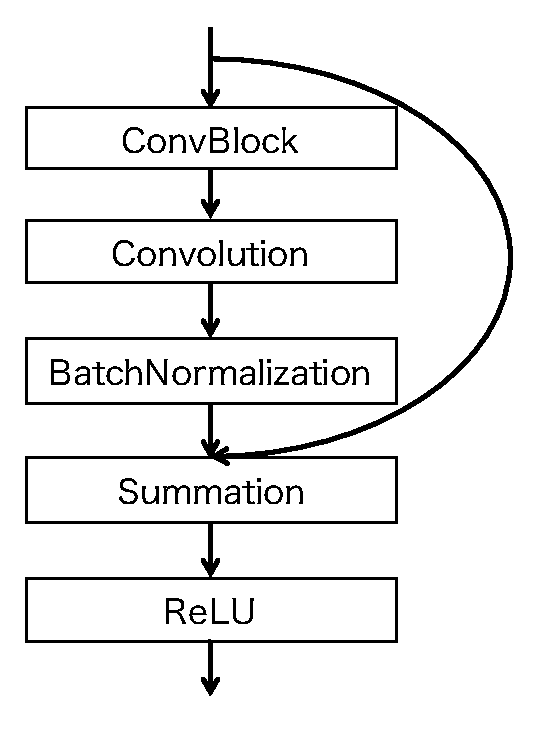
\includegraphics[scale=0.45]{images/resblock.eps}
\caption{ResBlock architecture.}
\label{resblock}
\end{figure}

% ----------------------------------------------------------------------------------------------------
\section{Experiments and Results}
\subsection{Dataset}
We test our method on the image classification task using the CIFAR-10 dataset in which the number of classes is $10$. The numbers of training and test images are $50,000$ and $10,000$, respectively, and the size of images is $32 \times 32$.

We consider two experimental scenarios: default scenario and small-data scenario.
The default scenario uses the default numbers of the training images, while the small-data scenario assumes that we only use $5,000$ images as the learning data. 

In the default scenario, we randomly sampled $45,000$ images from the training set to train the CNN and use the remaining $5,000$ images as the for the validation set for CGP fitness.
In the small-data scenario, we randomly sampled $4,500$ images for the training and $500$ images for the validation.

\subsection{Experimental Setting}

\begin{table}[t]
  \caption{Parameter settings for the CGP}
  \label{cgp_param}
  \begin{tabular}{l|l} \hline
    Parameters & Values \\ \hline
   \# Generations & $300$ \\ 
   Mutation rate & $0.05$ \\
   \#  Rows ($N_r$) & $5$ \\
   \#  Columns ($N_c$) & $30$ \\
   Levels-back ($l$) & $10$ \\ \hline
  \end{tabular}
\end{table}


To assign the fitness to the candidate CNN architectures, we train the CNN by stochastic gradient descent with the mini-batch size of $128$. The softmax cross entropy loss is used as the loss function.
We initialize the weights by the He's method \cite{he_delving_2015} and use the Adam optimizer \cite{kingma_adam:_2015} with an initial learning rate of $0.01$. 
Each CNN is trained for $50$ epochs and we reduce the learning rate by a factor of $10$ at $30$ epochs.

We preprocess the data with the per-pixel mean subtraction.
To prevent overfitting, we use weight decay with coefficient $1.0\times 10^{-4}$ and data augmentation.
We use the data augmentation method based on \todo{\cite{}}; padding $4$ pixels on each side followed by choosing a random $32\times 32$ crop from the padded image, and random horizontal flips on the cropped $32 \times 32$ image.

The parameter setting for the CGP is shown in Table \ref{cgp_param}. We use the relatively larger number of columns than the number of rows to generate deep architectures likely.
\shin{$\lambda ?$}

After the CGP process, we re-train the best CNN architecture using each training images ($50,000$ for the default scenario and $5,000$ for the small-data scenario) and calculate the classification accuracy for the $10,000$ test images to evaluate the constructed CNN architectures.
In this re-training phase, we optimize the weights of the obtained architecture with a different training schedule; we set a learning rate to $0.01$ during first $50$ epochs and then reduce to $0.001$ during subsequent $50$ epochs. The other parameters are same as used in the CGP process.
We run our experiments using Chianer \cite{tokui_chainer:_2015} on a machine with $3.2$GHz CPU, $32$GB RAM, and two NVIDIA GeForce GTX 1080 GPUs.

\shin{Checked up to here.}


\begin{figure*}[!t]
 \begin{minipage}[b]{0.45\linewidth}
  \centering
  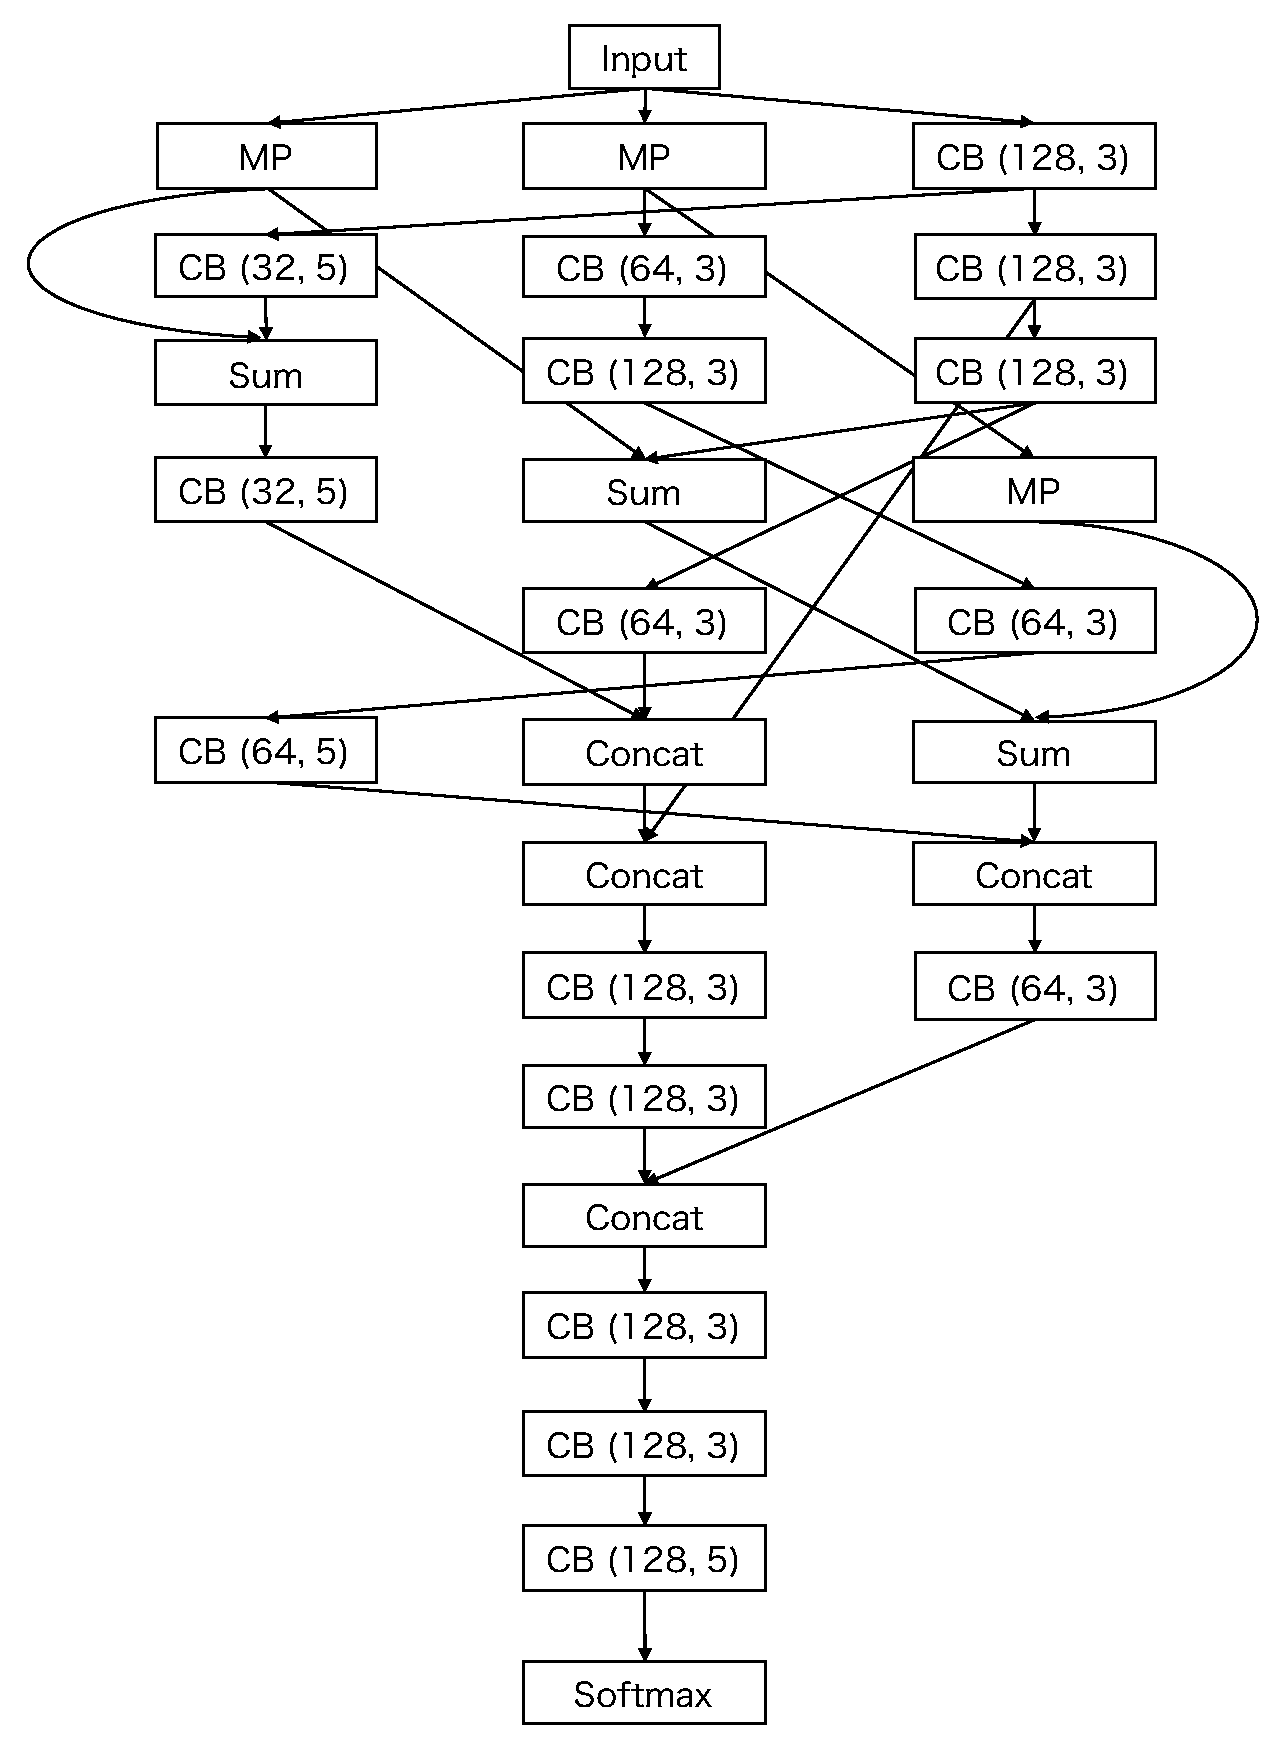
\includegraphics[keepaspectratio, scale=0.4]{images/modelA.eps}
  \subcaption{CGP-CNN (A)}\label{modelA}
 \end{minipage}
 \begin{minipage}[b]{0.45\linewidth}
  \centering
  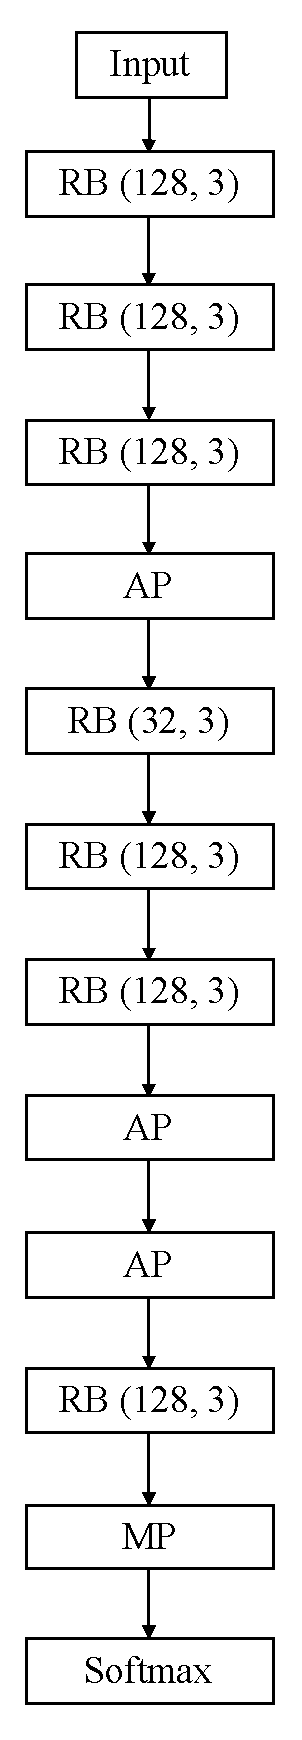
\includegraphics[keepaspectratio, scale=0.4]{images/modelB.eps}
  \subcaption{CGP-CNN (B)}\label{modelB}
 \end{minipage}
 \caption{Architectures designed by our method.}\label{models}
\end{figure*}

%\begin{figure*}[!t]
%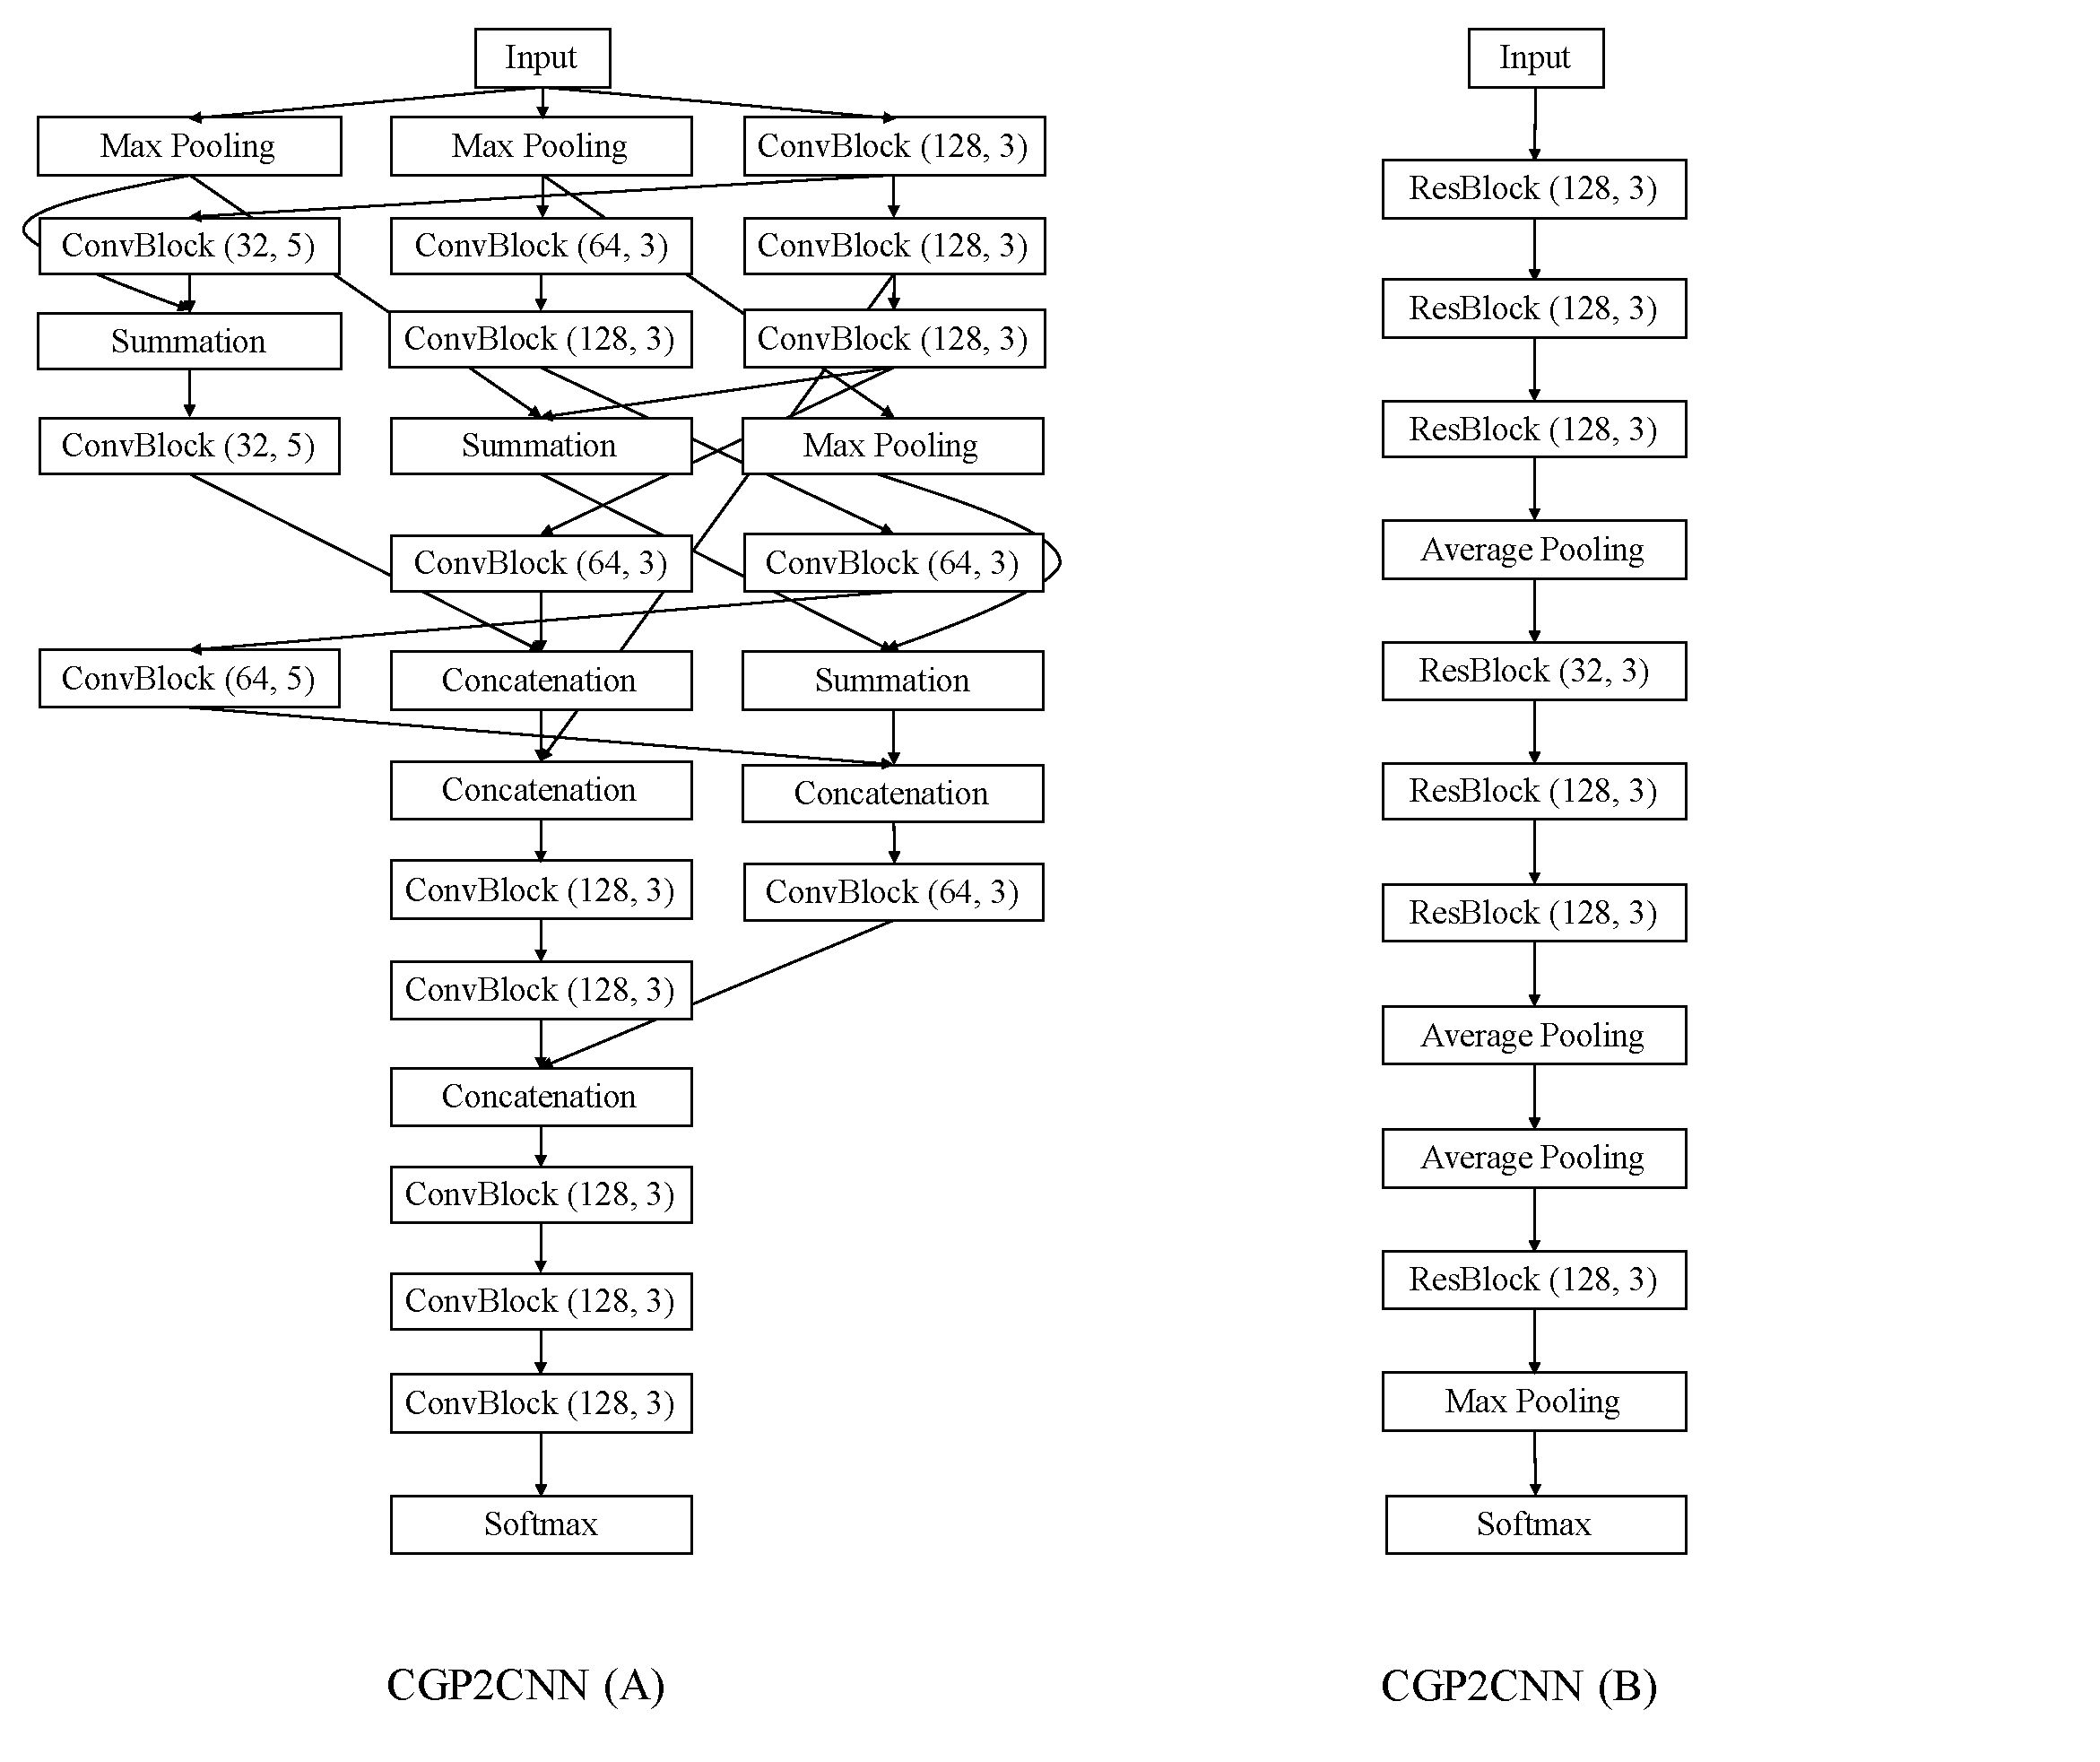
\includegraphics[scale=0.48]{images/models.eps}
%\caption{CNN architectures designed by our method. $ConvBlock(n, k)$ denotes a ConvBlock node with $n$ filters and receptive field size $k$. $ResBlock(n, k)$ denotes a ResBlock node with $n$ filters and receptive field size $k$.}
%\label{models}
%\end{figure*}

%\begin{figure}[!t]
%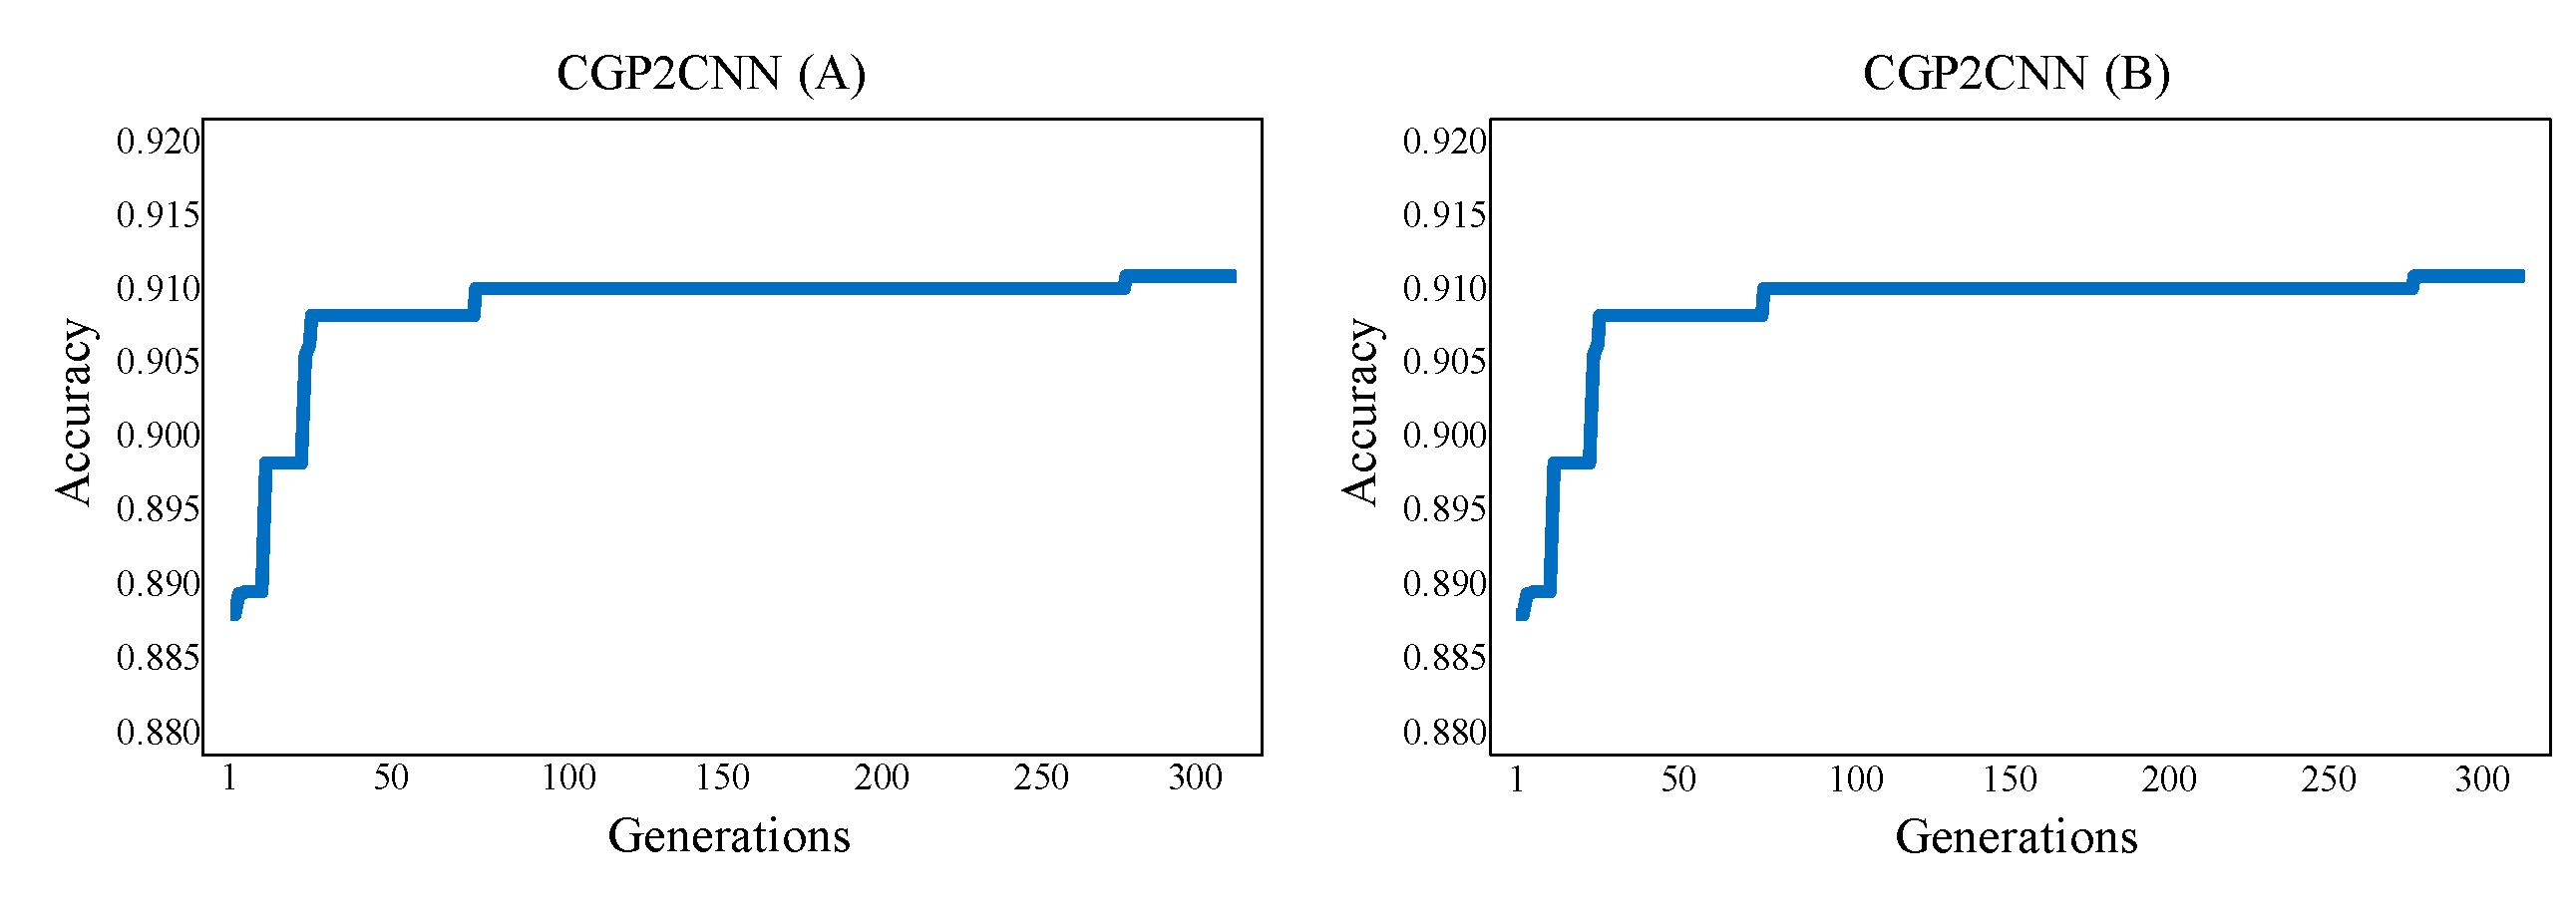
\includegraphics[scale=0.19]{images/fitness.eps}
%\caption{Transition of the fitness of CGP2CNN (A) and CGP2CNN (B).}
%\label{fitness}
%\end{figure}


\subsection{Results with the default scenario}
We compare the classification performance of our method with the state-of-the-art-methods and summarize the results in Table \ref{results}.
We refer to our architecture designed using the ConvBlock, max-pooling, average-pooling, summation, and concatenation functions as CGP-CNN (A) and the architecture using the ResBlock as an alternative to the ConvBlock as CGP-CNN (B).
As can be seen in Table \ref{results}, our results are competitive with the state-of-the-art-methods.
In particular, CGP-CNN (B) outperforms all hand-crafted models and our architectures have a good balance between classification accuracy and the number of parameters.
In this experiment, the architectures of CGP-CNN (A) and CGP-CNN (B) are quite different as seen in Figure \ref{models}.
For example, the summation and concatenation node are used frequently in CGP-CNN (A).
The nodes, on the other hand, are not used in CGP-CNN (B) but each model shows a good classification performance.
Added to this, we find that CGP-CNN (B) architecture has a similar features to the ResNet \cite{he_deep_2016}.
The architecture of the ResNet \cite{he_deep_2016} has several pairs of convolution layers and convolutions that performs downsampling with a stride of $2$.
Although our method cannot perform downsampling by convolution functions, we can see from Figure \ref{models} that CGP-CNN (B) uses average pooling as an alternative to the convolution layers for downsampling.
Furthermore, CGP-CNN (B) has some pairs of convolution nodes like the ResNet.
It follows from what has been said that our method also can design a architecture similar to one designed by human experts and its model shows a better performance.
Also, while the ResNet has a deep $110$-layer architecture, CGP-CNN (B) has a relatively shallow architecture and outperforms the ResNet.
We can see from this result that the number of output channels of the ResBlock is more effective than the depth at improving the classification accuracy on the CIFAR-10 dataset.

To explore the effectiveness of the number of output channels, we change the number of output channels CGP-CNN (A) can use from $\{32, 64, 128\}$ to $\{64, 128, 256, 512\}$ and refer to this model as CGP-CNN (C).
The result is improved to the error rate $7.25$\% and the CGP-CNN (C) has a more shallow architecture and fewer nodes than that of the CGP-CNN (A).


%The fitness transition of CGP2CNN (A) and CGP2CNN (B) is shown in Figure \ref{fitness}.
%While the fitness remains flat from $100$ generation to $250$ generation, the improvement of the fitness is seen in about $300$ generation.
%It is likely that our method shows a better classification performance if we train the CGP in more generations.


\begin{table}[t]
  \caption{Comparison of error rate on CIFAR-10 dataset.}
  \label{results}
  \begin{tabular}{l|c|c} \hline
    Model & Error rate & \# params ($10^6$) \\ \hline
   Maxout \cite{goodfellow_maxout_2013} & $9.38$ & - \\ 
   MetaQNN \cite{baker_designing_2016} \footnotemark & $9.09$ & $3.7$ \\
   Network in Network \cite{lin_network_2013} & $8.81$ & - \\
   VGG \cite{simonyan_very_2014} \footnotemark & $7.94$ & $15.2$ \\
   CGP-CNN (A) & $7.89$ & $1.52$ \\
   ResNet \cite{he_deep_2016} & $6.61$ & $1.7$ \\
   CGP-CNN (B) & $5.98$ & $1.68$ \\
   Neural Architecture Search \cite{zoph_neural_2016} & $3.84$ & $32.0$ \\ \hline
   %\multicolumn{1}{l}{*The mean error rate and the number of parameters of top $5$ models.} & \multicolumn{1}{l}{} & \multicolumn{1}{l}{} \\
  \end{tabular}
\end{table}
\footnotetext[1]{The mean error rate and the number of parameters of top $5$ models are shown.}
\footnotetext[2]{We implemented the VGG net \cite{simonyan_very_2014} and applied the model to the CIFAR-10 dataset since the 
VGG net is not applied to the CIFAR-10 dataset in \cite{simonyan_very_2014}.
The architecture of the VGG is identical with the configuration D in \cite{simonyan_very_2014}.
We denote this model as VGG in this paper.}


\subsection{Results with the small-data scenario}
For settings of our method, we changed the number of generation to $2,000$.
The other experimental settings are the same in the preceding section.
In this experiment, we compare our method with the VGG and ResNet.
For the VGG settings, the VGG is trained for $200$ epochs with SGD with an initial learning rate of $0.01$.
We reduce the learning rate by a factor of $10$ every $50$ epochs.
For the ResNet, we train the model for $500$ epochs.
We use SGD and start with a learning rate of $0.1$, then divide it by $10$ at $250$ and $375$ epochs.

Table \ref{results_small} shows that our model can find better architectures than the VGG and ResNet.
The CGP-CNN (A) architecture is shown in Figure \ref{model_small}.
As seen in Figure \ref{model_small}, our method discovers the structure different from that in the preceding section.
In addition, we retrain this model with $50,000$ training images and then compute the test accuracy, and achieves $9.2\%$ error rate on the test set.
We can see from these experiments that even with a small dataset, our method can design a relatively good architecture.


\begin{table}[t]
  \caption{Comparison of error rate with the small CIFAR-10 dataset.}
  \label{results_small}
  \begin{tabular}{l|c|c} \hline
    Model & Error rate & \# params ($10^6$) \\ \hline
   VGG \cite{simonyan_very_2014} & $27.67$ & 15.2 \\
   CGP-CNN (B) & $24.50$ & $0.91$ \\ 
   ResNet \cite{he_deep_2016} & $24.10$ & 1.7 \\ 
   CGP-CNN (A) & $22.82$  & $3.9$  \\ \hline
  \end{tabular}
\end{table}

\begin{figure}[t]
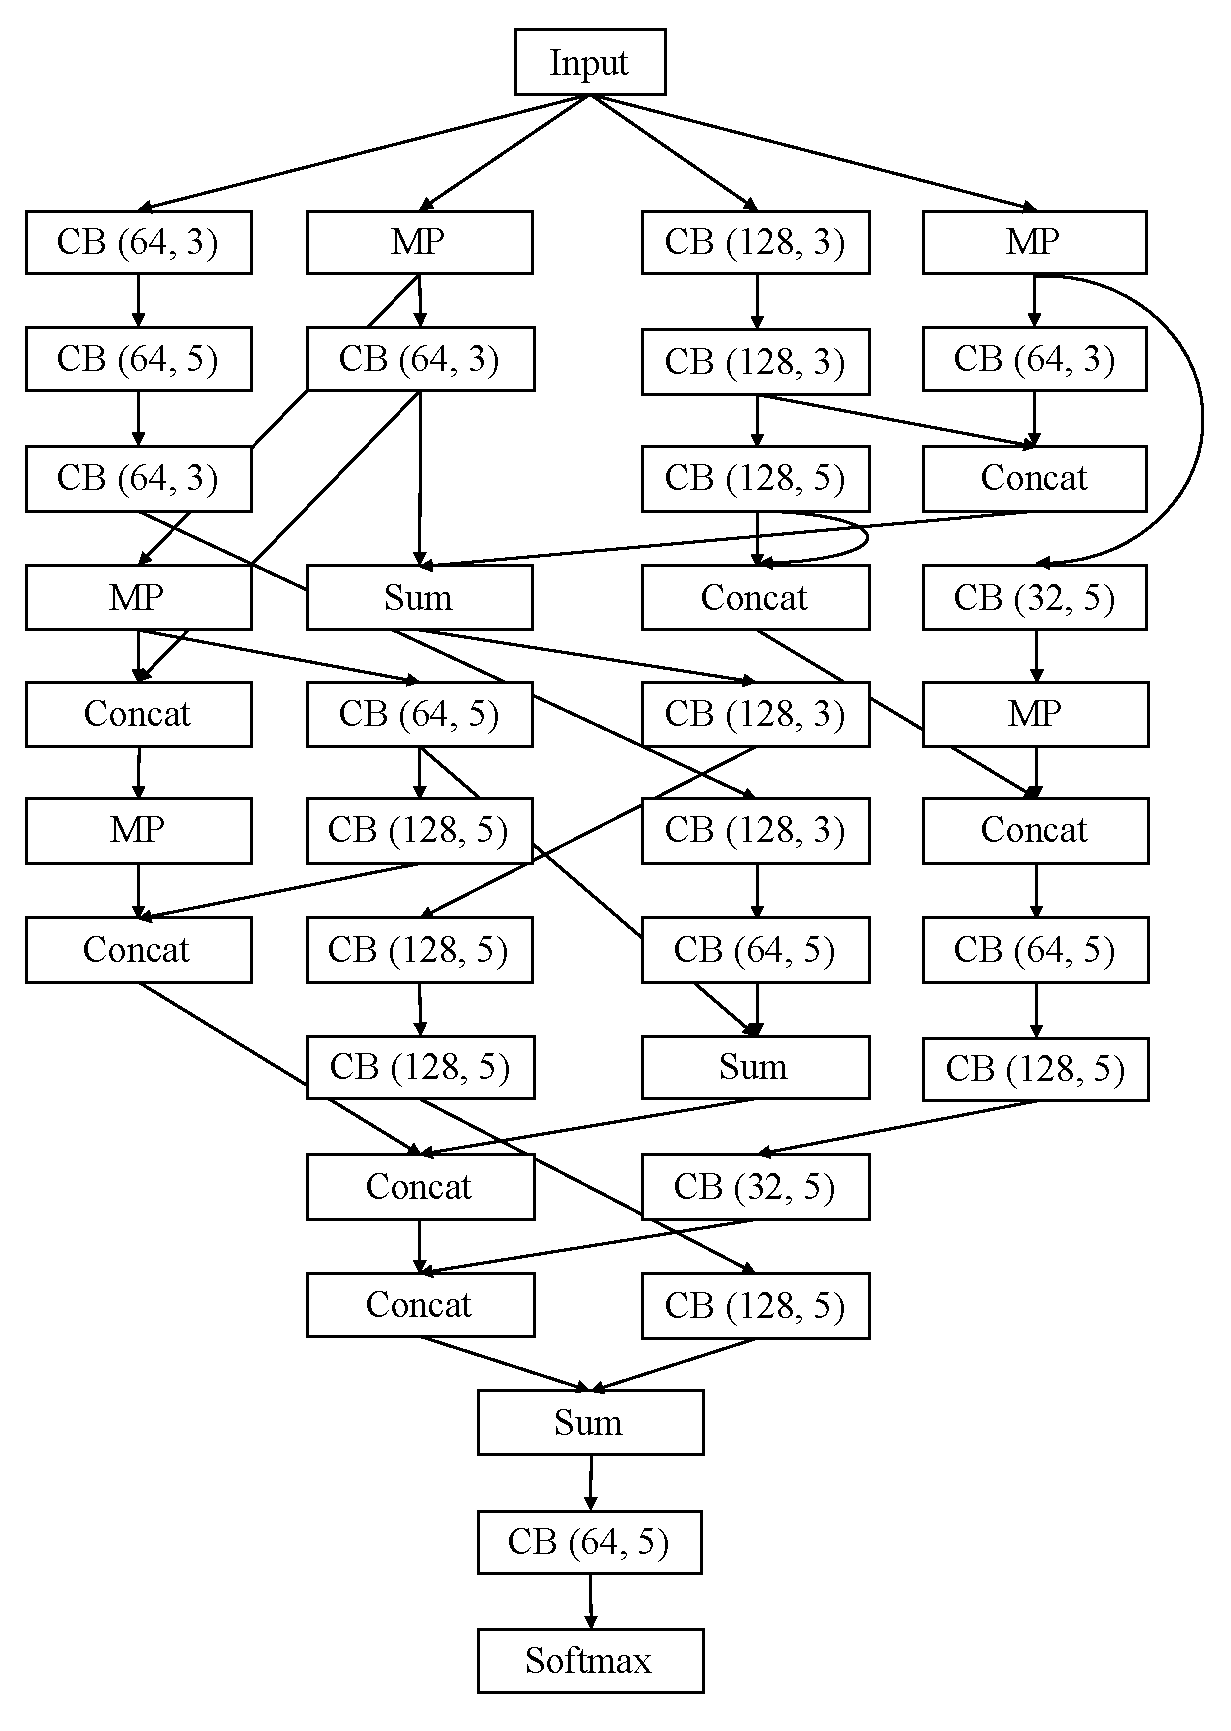
\includegraphics[scale=0.35]{images/model_small.eps}
\caption{The architecture of CGP-CNN (A) with the small-data scenario.}
\label{model_small}
\end{figure}


\section{Conclusions}
In this paper we propose a GP-based method for designing CNN architectures and show that our method is able to deign competitive models compared with state-of-the-art method on the image classification task. 
By using a highly-functional modules such as ConvBlock and ResBlock, our method achieves a high performance and efficient optimization.

In our future work, we will evaluate our method with a more challenging task.
Also, we will improve optimization cost of our method because our method take about a week to design architectures in this experiment.
